\documentclass[xetex,mathserif,serif]{beamer}
\usepackage{polyglossia}
\setdefaultlanguage[babelshorthands=true]{russian}
\usepackage{minted}
\usepackage{tabu}

\useoutertheme{infolines}

\usepackage{fontspec}
\setmainfont{FreeSans}
\newfontfamily{\russianfonttt}{FreeSans}

\definecolor{links}{HTML}{2A1B81}
\hypersetup{colorlinks,linkcolor=,urlcolor=links}

\tabulinesep=0.7mm

\newcommand{\attribution}[1] {
    \vspace{-5mm}\begin{flushright}\begin{scriptsize}\textcolor{gray}{\textcopyright\, #1}\end{scriptsize}\end{flushright}
}

\title{Лекция 15: Примеры архитектур}
\author[Юрий Литвинов]{Юрий Литвинов\\\small{\textcolor{gray}{y.litvinov@spbu.ru}}}

\date{21.12.2021}

\begin{document}

    \frame{\titlepage}
    \section{Enterprise Fizz-Buzz}

    \begin{frame}
        \frametitle{Enterprise Fizz-Buzz}
        Задача:

        Для чисел от 1 до 100:
        \begin{itemize}
            \item если число делится на 3, вывести ``Fizz''
            \item если число делится на 5, вывести ``Buzz''
            \item если число делится и на 3, и на 5, вывести ``FizzBuzz''
            \item во всех остальных случаях вывести само число
        \end{itemize}

        Решение:

        \url{https://github.com/EnterpriseQualityCoding/FizzBuzzEnterpriseEdition}
    \end{frame}

    \begin{frame}
        \frametitle{Структура системы}
        \begin{center}
            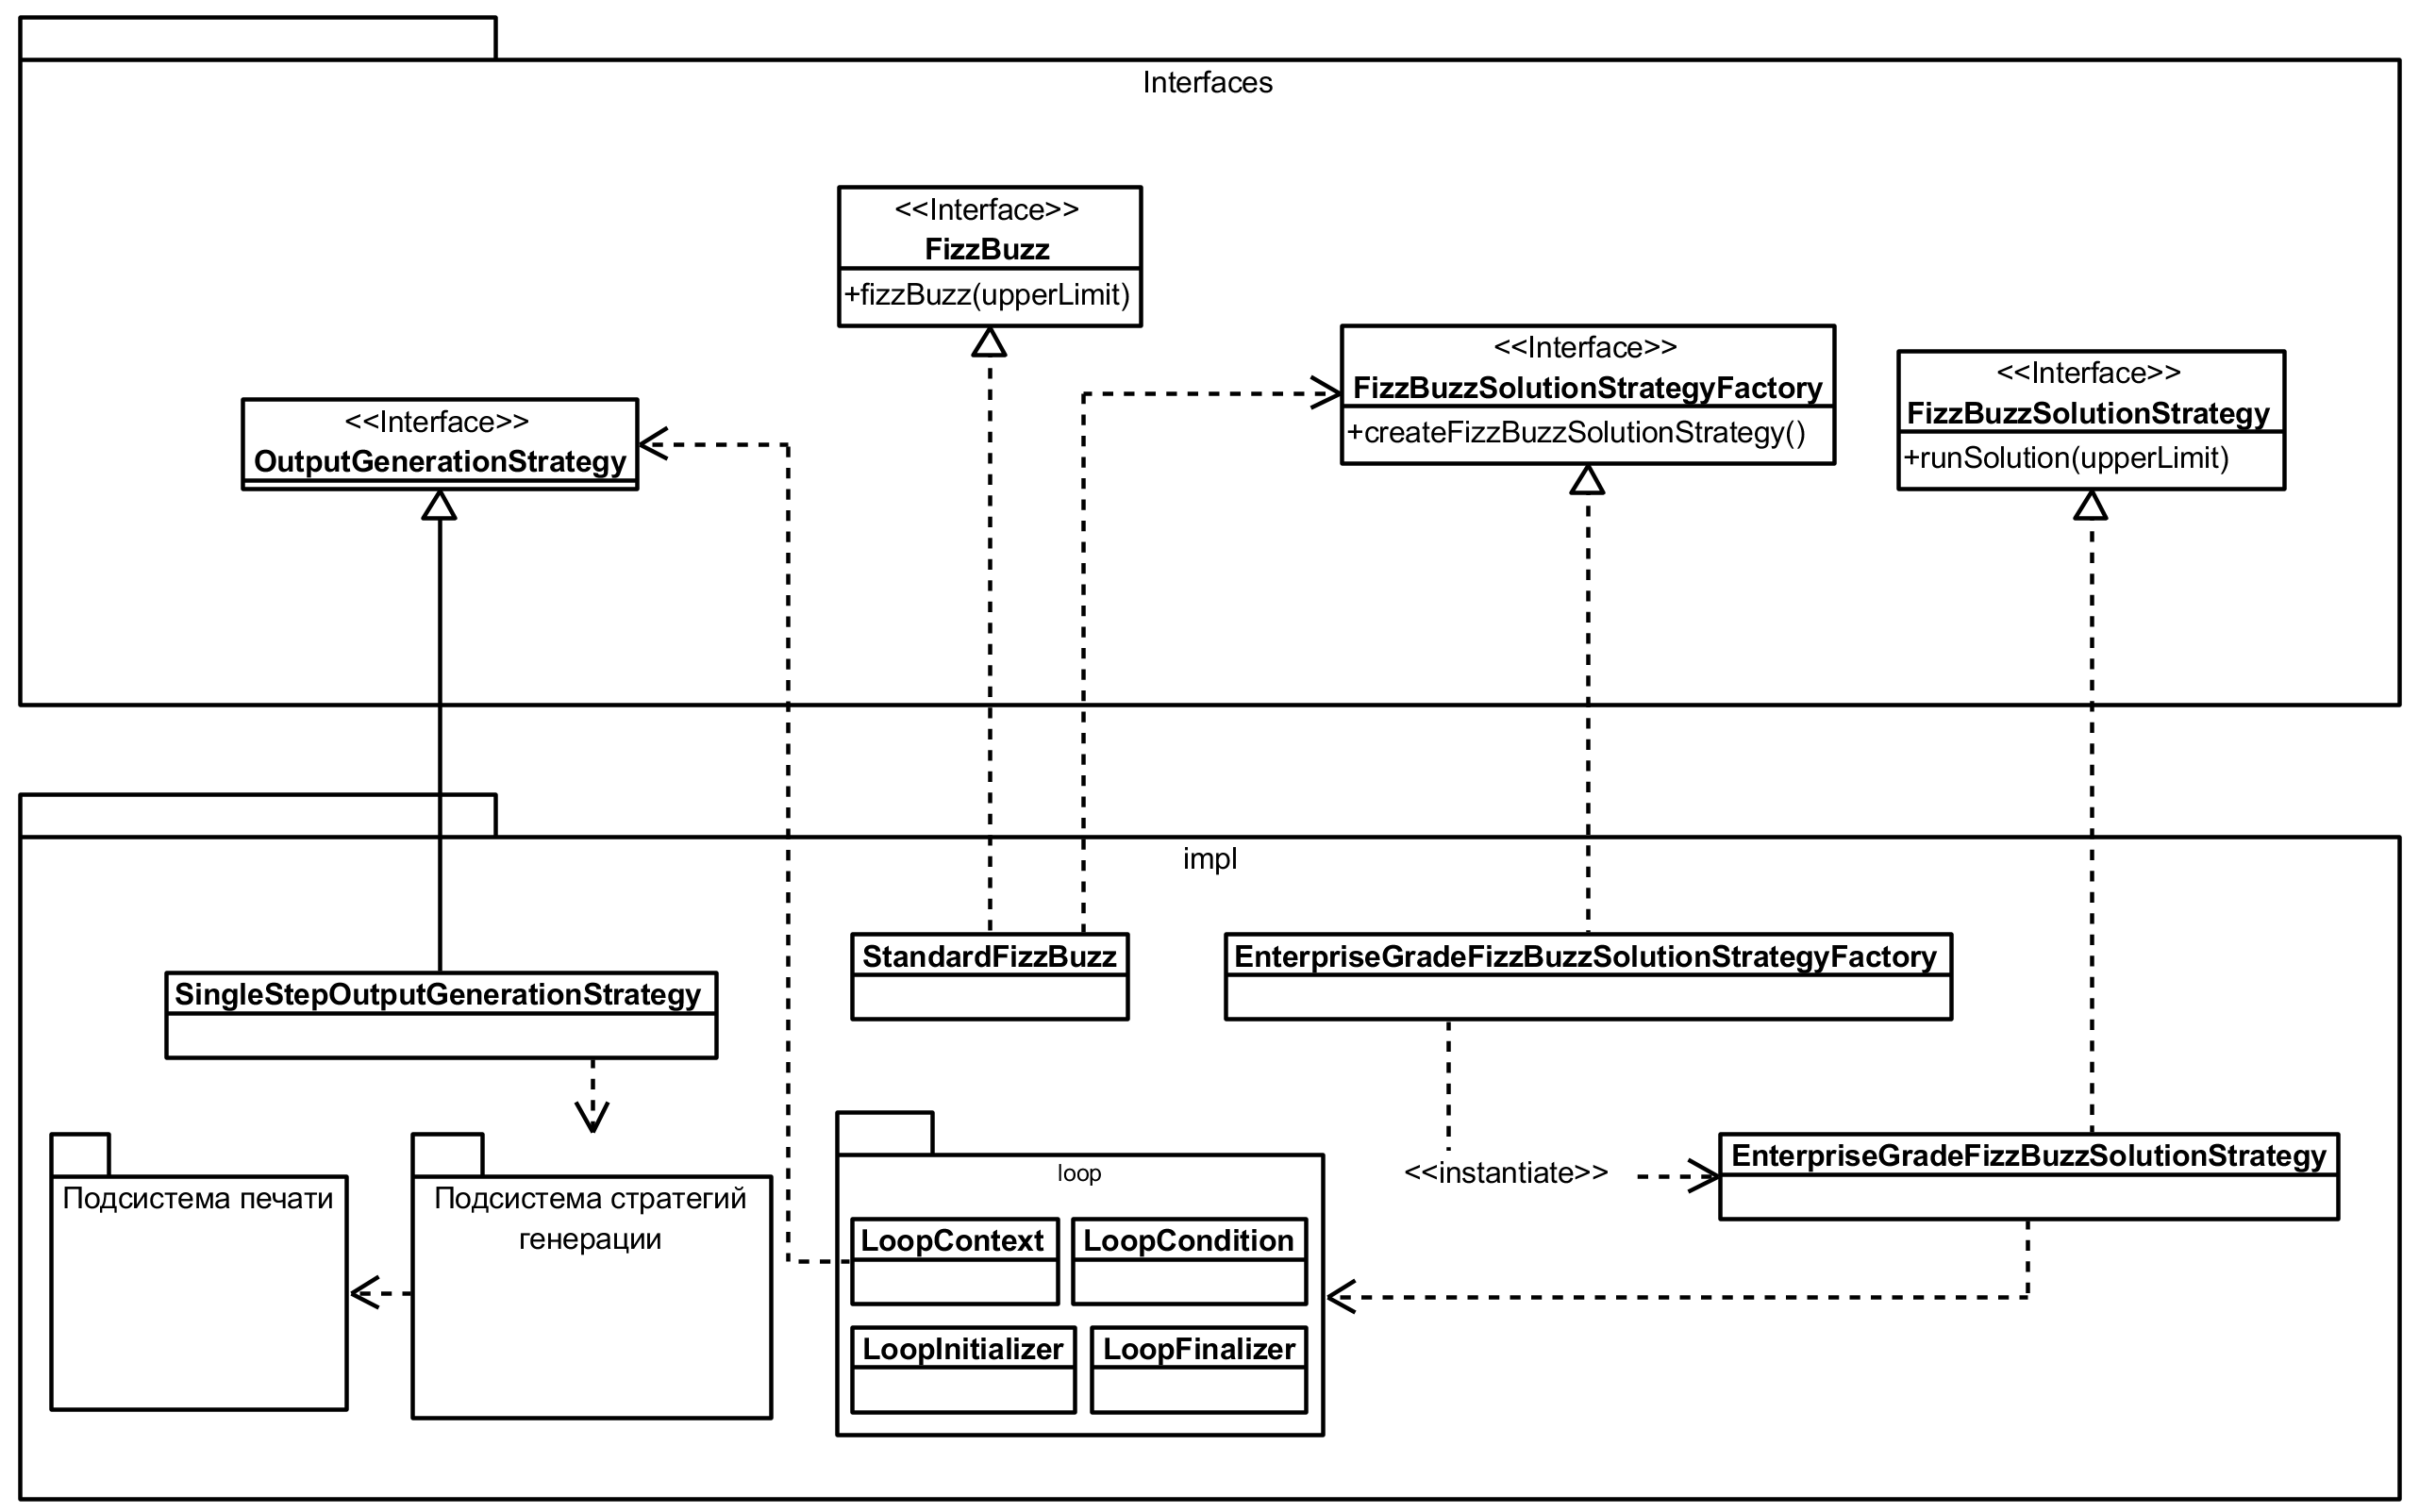
\includegraphics[width=\textwidth]{fizzBuzzArchitecture.png}
        \end{center}
    \end{frame}

    \begin{frame}
        \frametitle{Хорошие идеи}
        \begin{itemize}
            \item Separation of Concerns
            \item Dependency Inversion
            \item Dependency Injection
            \begin{itemize}
                \item Spring Framework
            \end{itemize}
            \item Паттерны ``Фабрика'', ``Стратегия'', ``Посетитель'', ``Адаптер'', что-то вроде паттернов ``Спецификация'' и ``Цепочка ответственности''
        \end{itemize}
    \end{frame}

    \begin{frame}
        \frametitle{Плохие идеи}
        \begin{itemize}
            \item Не выполняется принцип Keep It Simple Stupid
            \begin{itemize}
                \item Неправильно говорить ``строк кода написано'', правильно --- ``строк кода израсходовано''
            \end{itemize}
            \item ``Синтаксическое'' разделение на пакеты, а не ``семантическое''
            \begin{itemize}
                \item Отсуствие модульности, антипаттерн ``Big Ball of Mud''
            \end{itemize}
            \item Хардкод основных параметров вычисления
            \item Нет юнит-тестов, только интеграционные; нет логирования
            \item 1663 строки кода и всего 40 строк комментариев
            \begin{itemize}
                \item Отсутствие архитектурного описания
            \end{itemize}
        \end{itemize}
    \end{frame}

    \section{Bash}

    \begin{frame}
        \frametitle{Bash}
        \begin{itemize}
            \item Примерно 70К строк кода
            \item Исходный автор --- Brian Fox, maintainer --- Chet Ramey
            \item Первый релиз --- 1989
            \item Написан на C
            \item Архитектурное описание --- глава в \textit{The Architecture of Open Source Applications}, написанная Chet Ramey
        \end{itemize}
    \end{frame}

    \begin{frame}
        \frametitle{Архитектура Bash}
        \begin{center}
            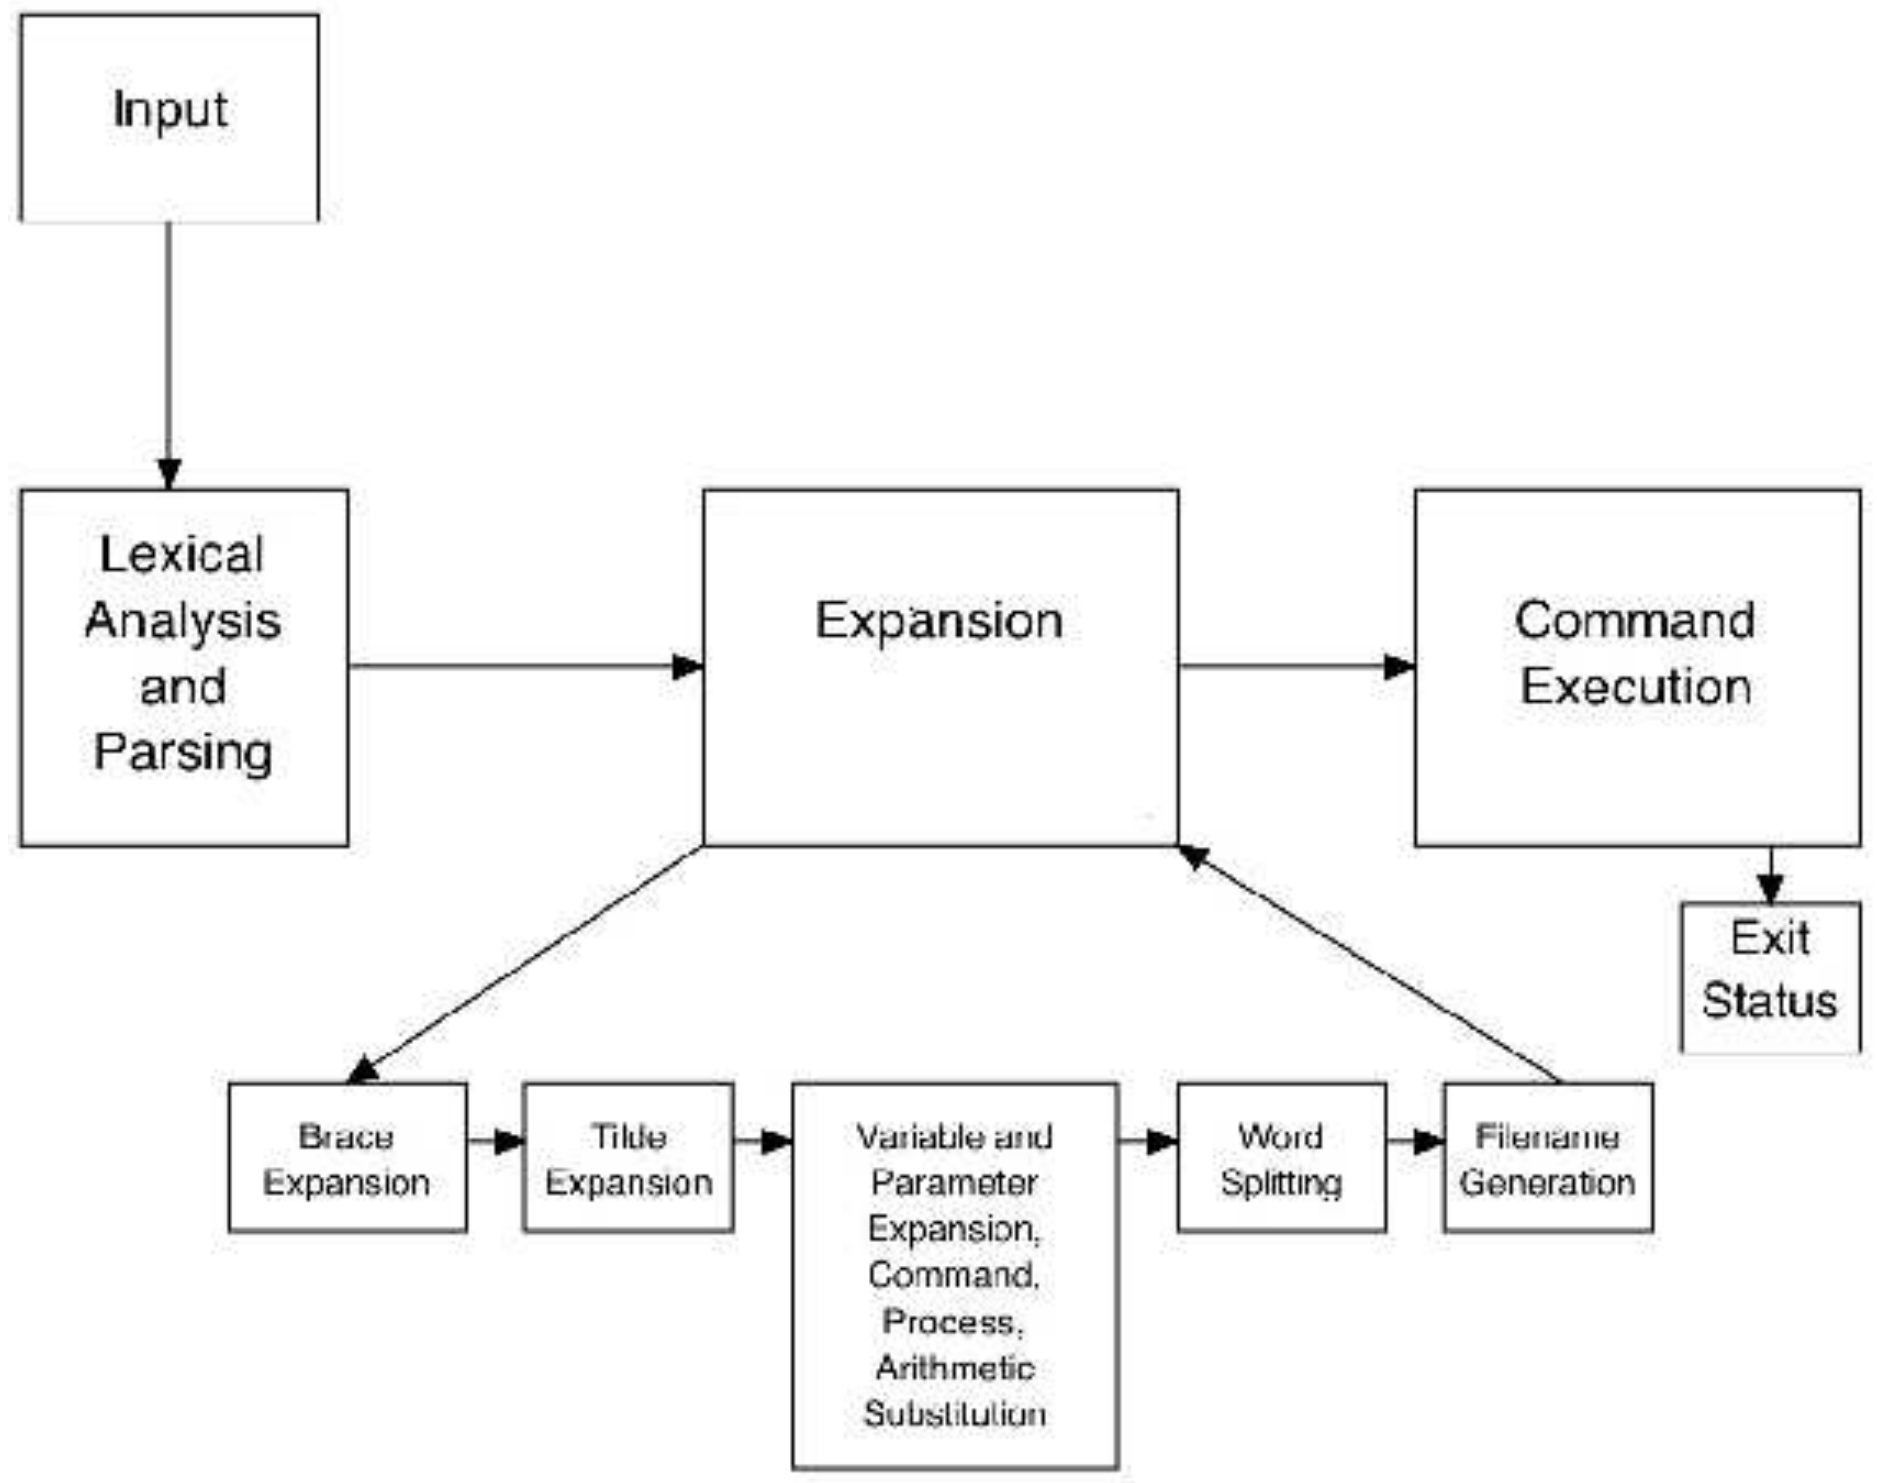
\includegraphics[width=0.7\textwidth]{bashArchitecture.png}
        \end{center}
    \end{frame}

    \begin{frame}[fragile]
        \frametitle{Основные структуры данных}
        \begin{minted}{c}
typedef struct word_desc {
    char *word; /* Zero terminated string. */
    int flags; /* Flags associated with this word. */
} WORD_DESC;
        \end{minted}

        \vspace{3mm}

        \begin{minted}{c}
typedef struct word_list {
    struct word_list *next;
    WORD_DESC *word;
} WORD_LIST;
        \end{minted}
    \end{frame}

    \begin{frame}
        \frametitle{Ввод с консоли}
        \begin{itemize}
            \item Библиотека Readline
            \begin{itemize}
                \item независимая библиотека, но пишется в основном для Bash
            \end{itemize}
            \item Цикл read/dispatch/execute/redisplay
            \item Dispatch table (или Keymap)
            \item Буфер редактирования, хитрый механизм расчёта действий для отображения
            \item Хранит все данные как 8-битные символы, но знает про Unicode
        \end{itemize}
    \end{frame}

    \begin{frame}[fragile]
        \frametitle{Синтаксический разбор}
        \begin{itemize}
            \item Зависимый от контекста лексический анализ
                \begin{minted}{sh}
for for in for; do for=for; done; echo $for
                \end{minted}
            \item Использует lex + bison
            \item Подстановка alias-ов выполняется лексером
            \item Сохранение и восстановление состояния парсера
        \end{itemize}
    \end{frame}

    \begin{frame}[fragile]
        \frametitle{Подстановки}
        \begin{minted}{sh}
${parameter:-word}
        \end{minted}

раскрывается в \textit{parameter}, если он установлен, и в \textit{word}, если нет

        \begin{minted}{sh}
pre{one,two,three}post
        \end{minted}

раскрывается в 

        \begin{minted}{sh}
preonepost pretwopost prethreepost
        \end{minted}

        Ещё бывает подстановка тильды и арифметическая подстановка, сопоставление шаблона
    \end{frame}

    \begin{frame}[fragile]
        \frametitle{Исполнение команд}
        \begin{itemize}
            \item Встроенные и внешние команды, обрабатываются единообразно
            \item Перенаправление ввода-вывода, отмена перенаправления
            \item Принимают набор слов
            \begin{itemize}
                \item Иногда обрабатывают по-особому, например, присваивание в \textit{export}
            \end{itemize}
            \item Присваивание --- тоже команда, но особая
            \item Перед запуском внешней команды --- поиск в PATH, кеширование результатов
            \item Job control, foreground и background
        \end{itemize}
    \end{frame}

    \begin{frame}[fragile]
        \frametitle{Lessons Learned}
        \begin{itemize}
            \item Комментарии к коммитам со ссылками на багрепорты с шагами воспроизведения
            \item Хороший набор тестов, в Bash их тысячи
            \item Стандарты, как внешние на функциональность шелла, так и на код
            \item Пользовательская документация
            \item Переиспользование
        \end{itemize}
    \end{frame}

    \section{Bash, на самом деле}

    \begin{frame}
        \frametitle{Архитектура Bash, на самом деле}
        \begin{itemize}
            \item J. Garcia et al., \textit{Obtaining Ground-Truth Software Architectures}
            \item 1 аспирант, 80 часов работы
            \item Верификация от Chet Ramey
            \item 70К строк кода, 200 файлов, 25 компонент
            \begin{itemize}
                \item 16 --- ядро, 9 --- утилиты
            \end{itemize}
            \item Структура папок почти не соответствует выделенным компонентам
        \end{itemize}
    \end{frame}

    \begin{frame}
        \frametitle{Архитектура Bash, на самом деле}
        \begin{center}
            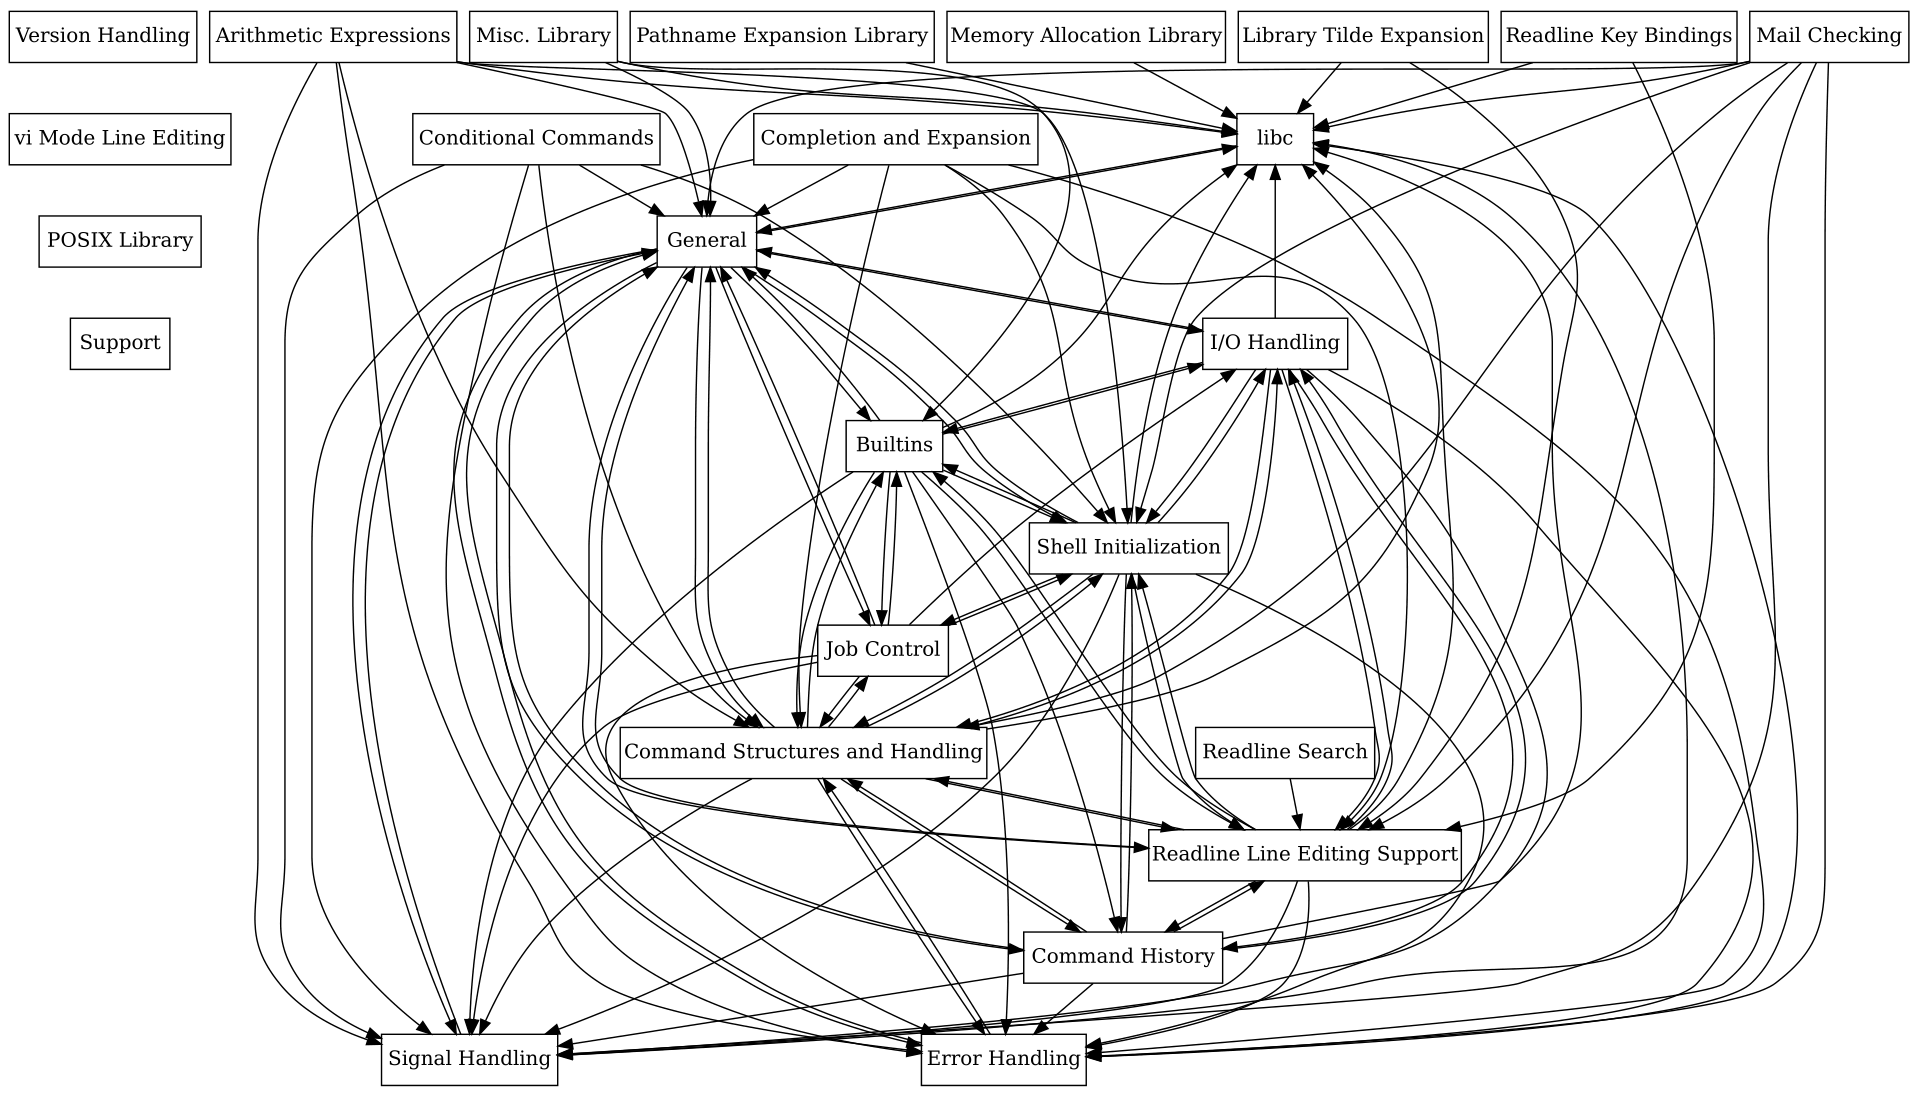
\includegraphics[width=\textwidth]{bashRealArchitecture.png}
        \end{center}
    \end{frame}

    \begin{frame}
        \frametitle{Результаты анализа кода}
        \begin{center}
            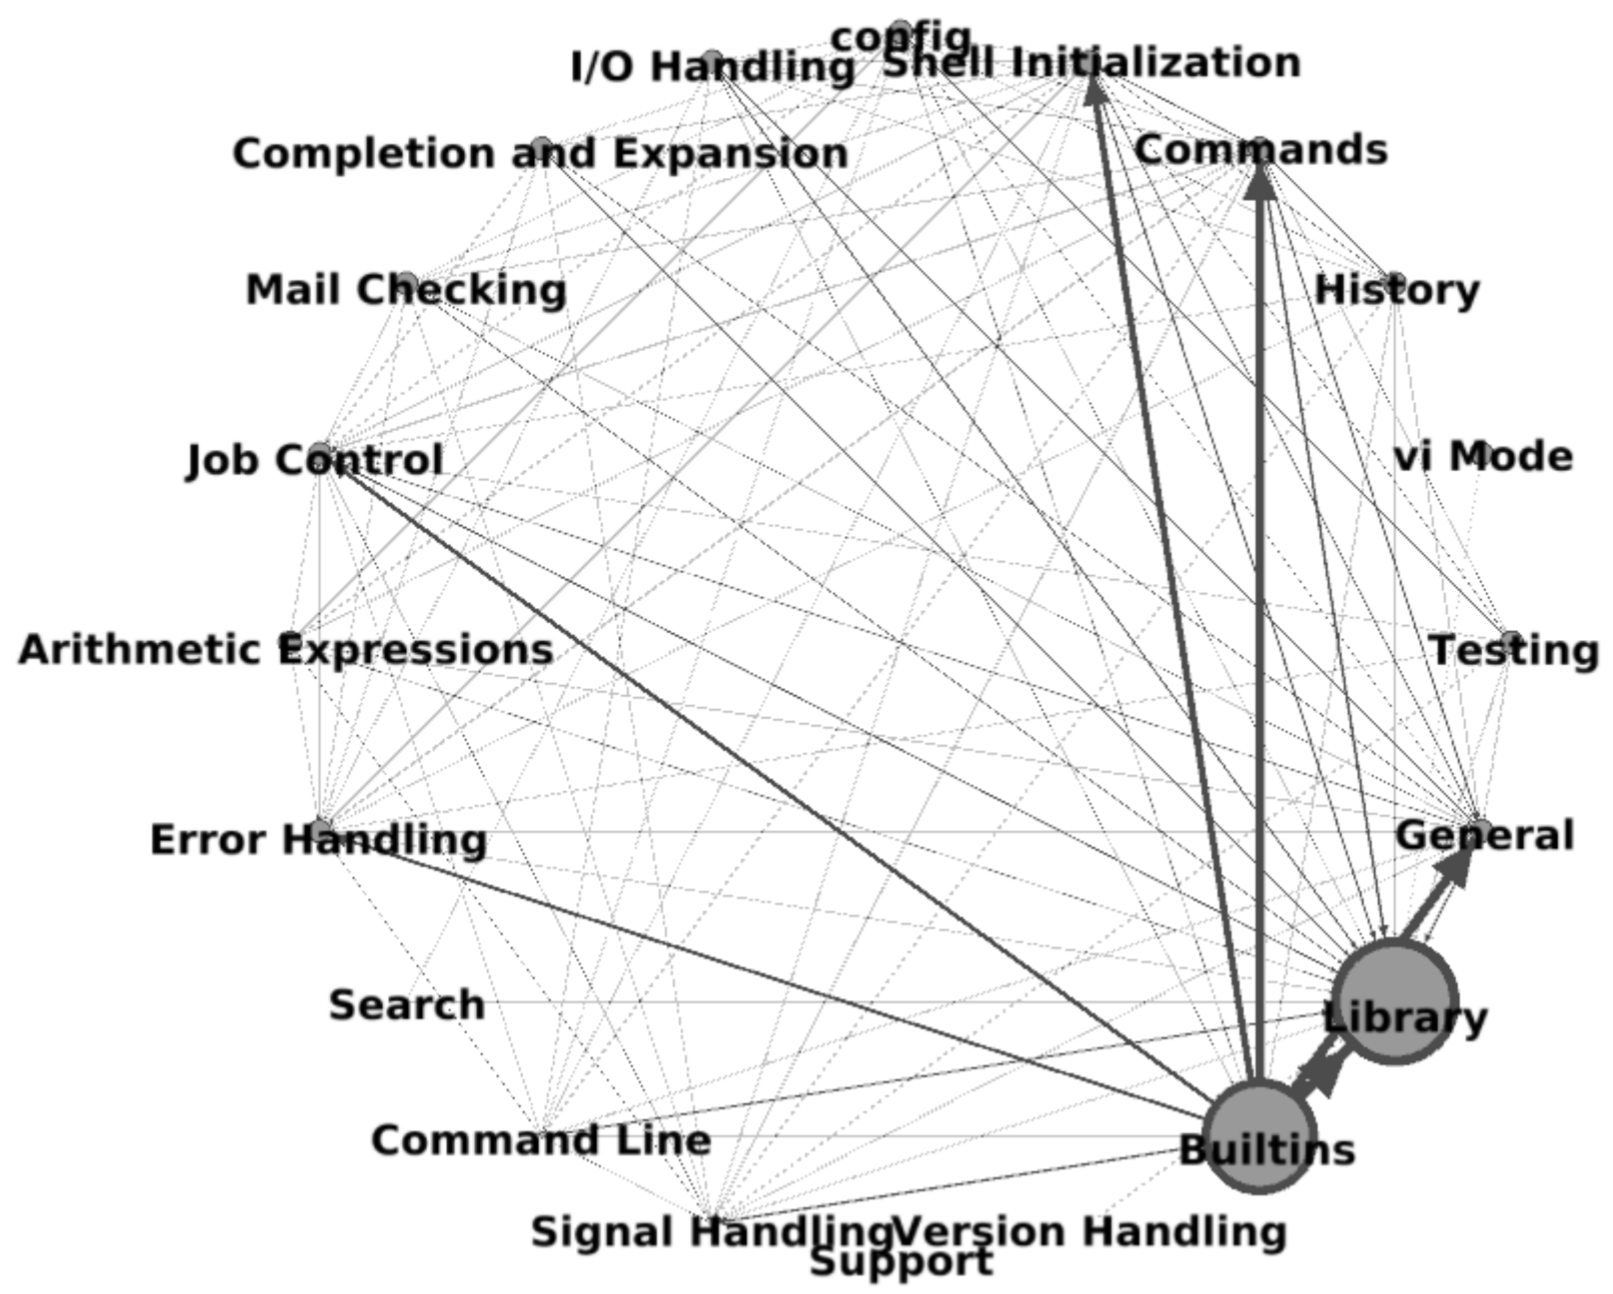
\includegraphics[width=0.7\textwidth]{bashAutomaticRecoveryArchitecture.png}
        \end{center}
    \end{frame}

    \begin{frame}
        \frametitle{Сравним с исходной}
        \begin{center}
            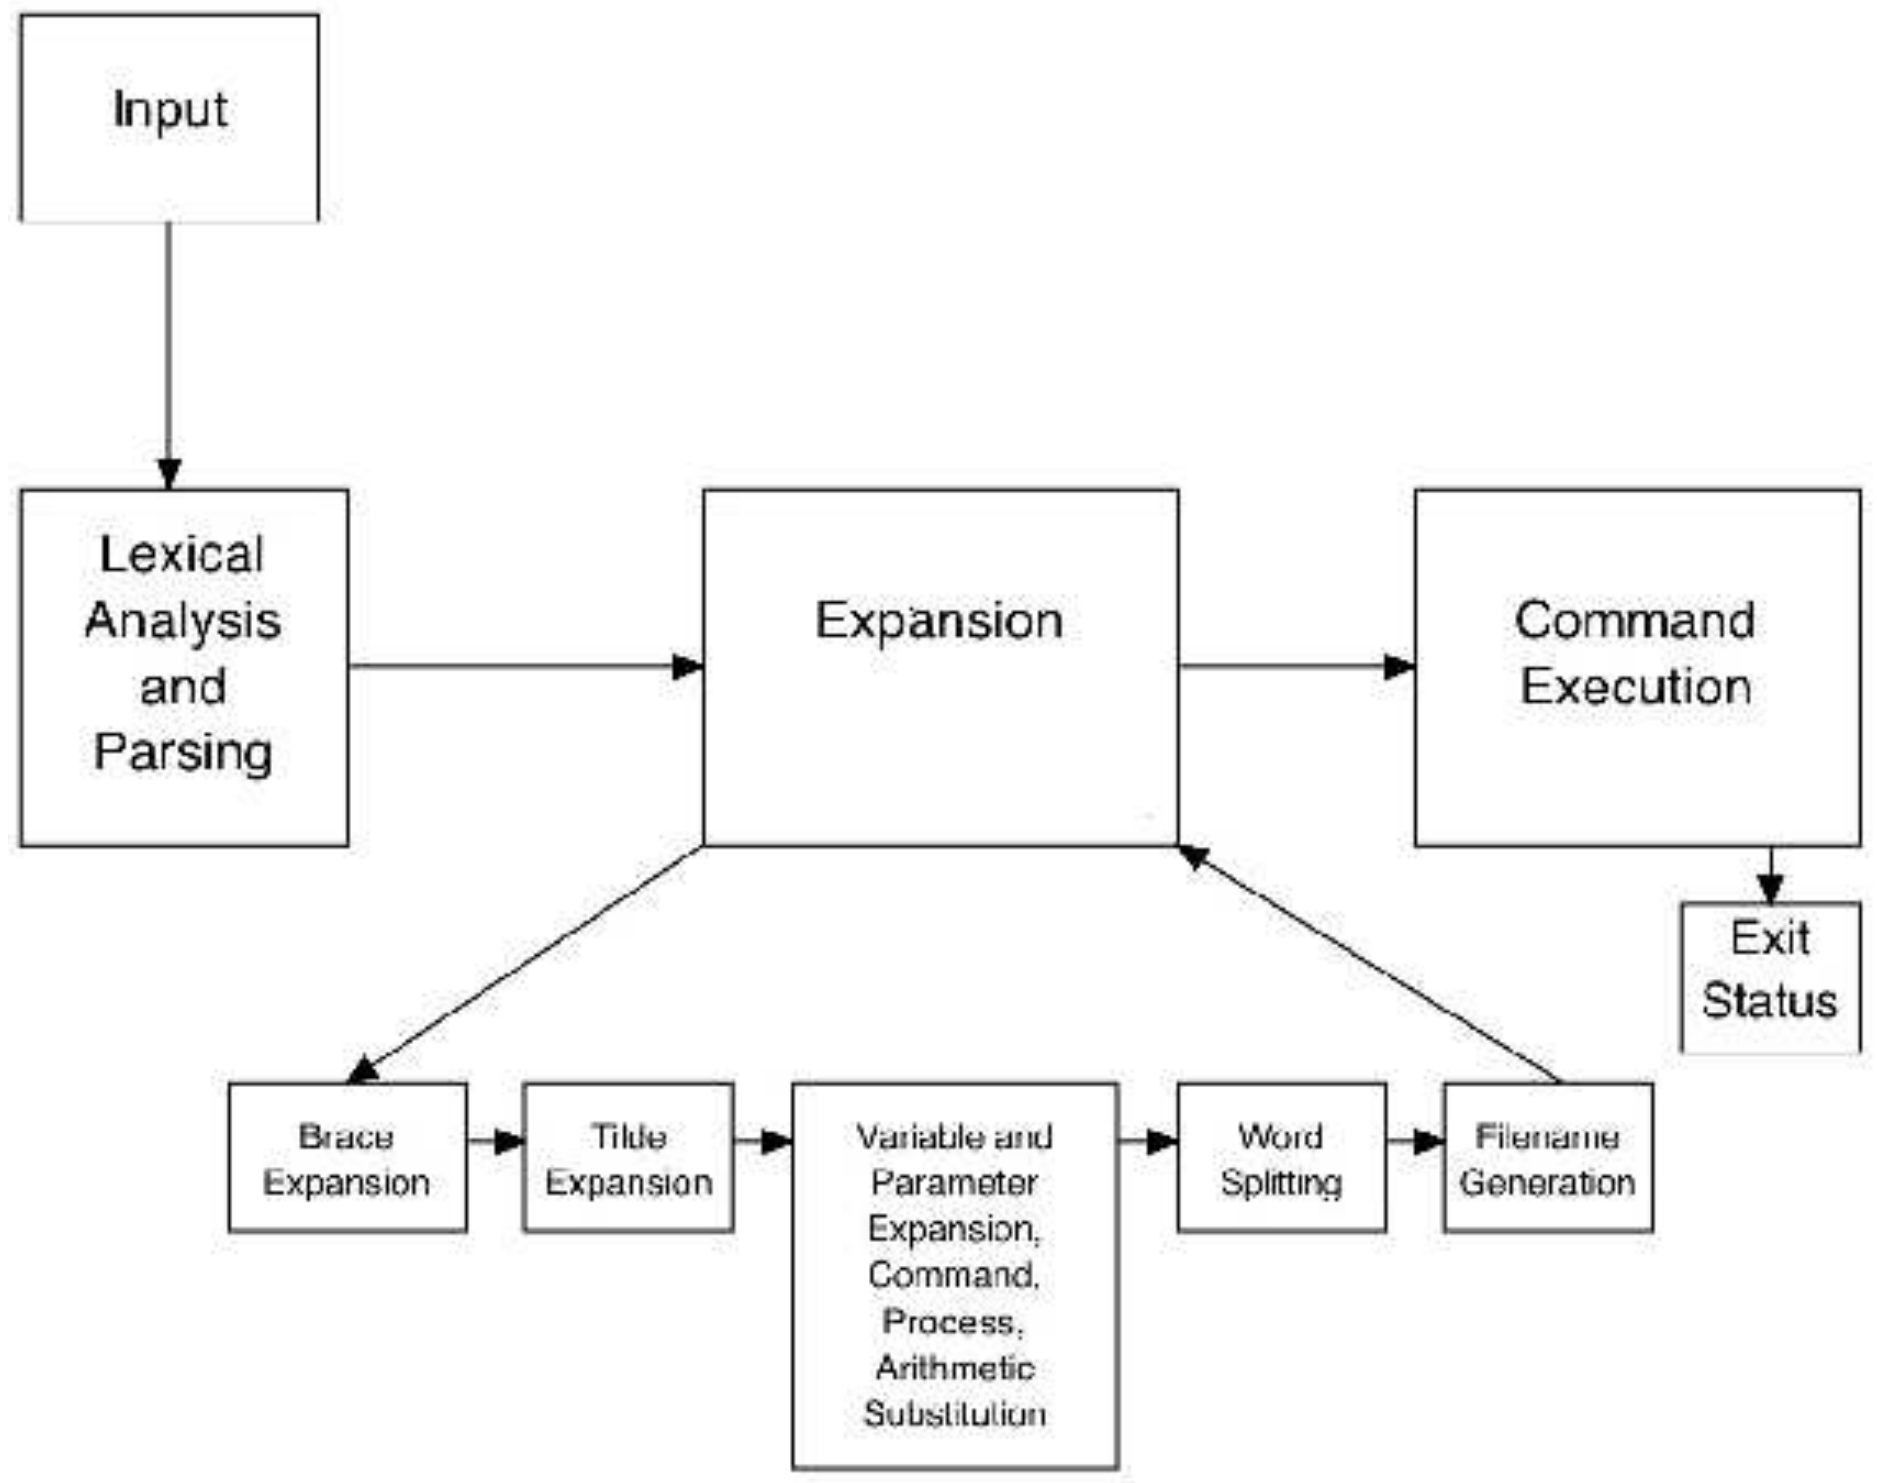
\includegraphics[width=0.7\textwidth]{bashArchitecture.png}
        \end{center}
    \end{frame}

    \begin{frame}
        \frametitle{Job Control}
        \begin{center}
            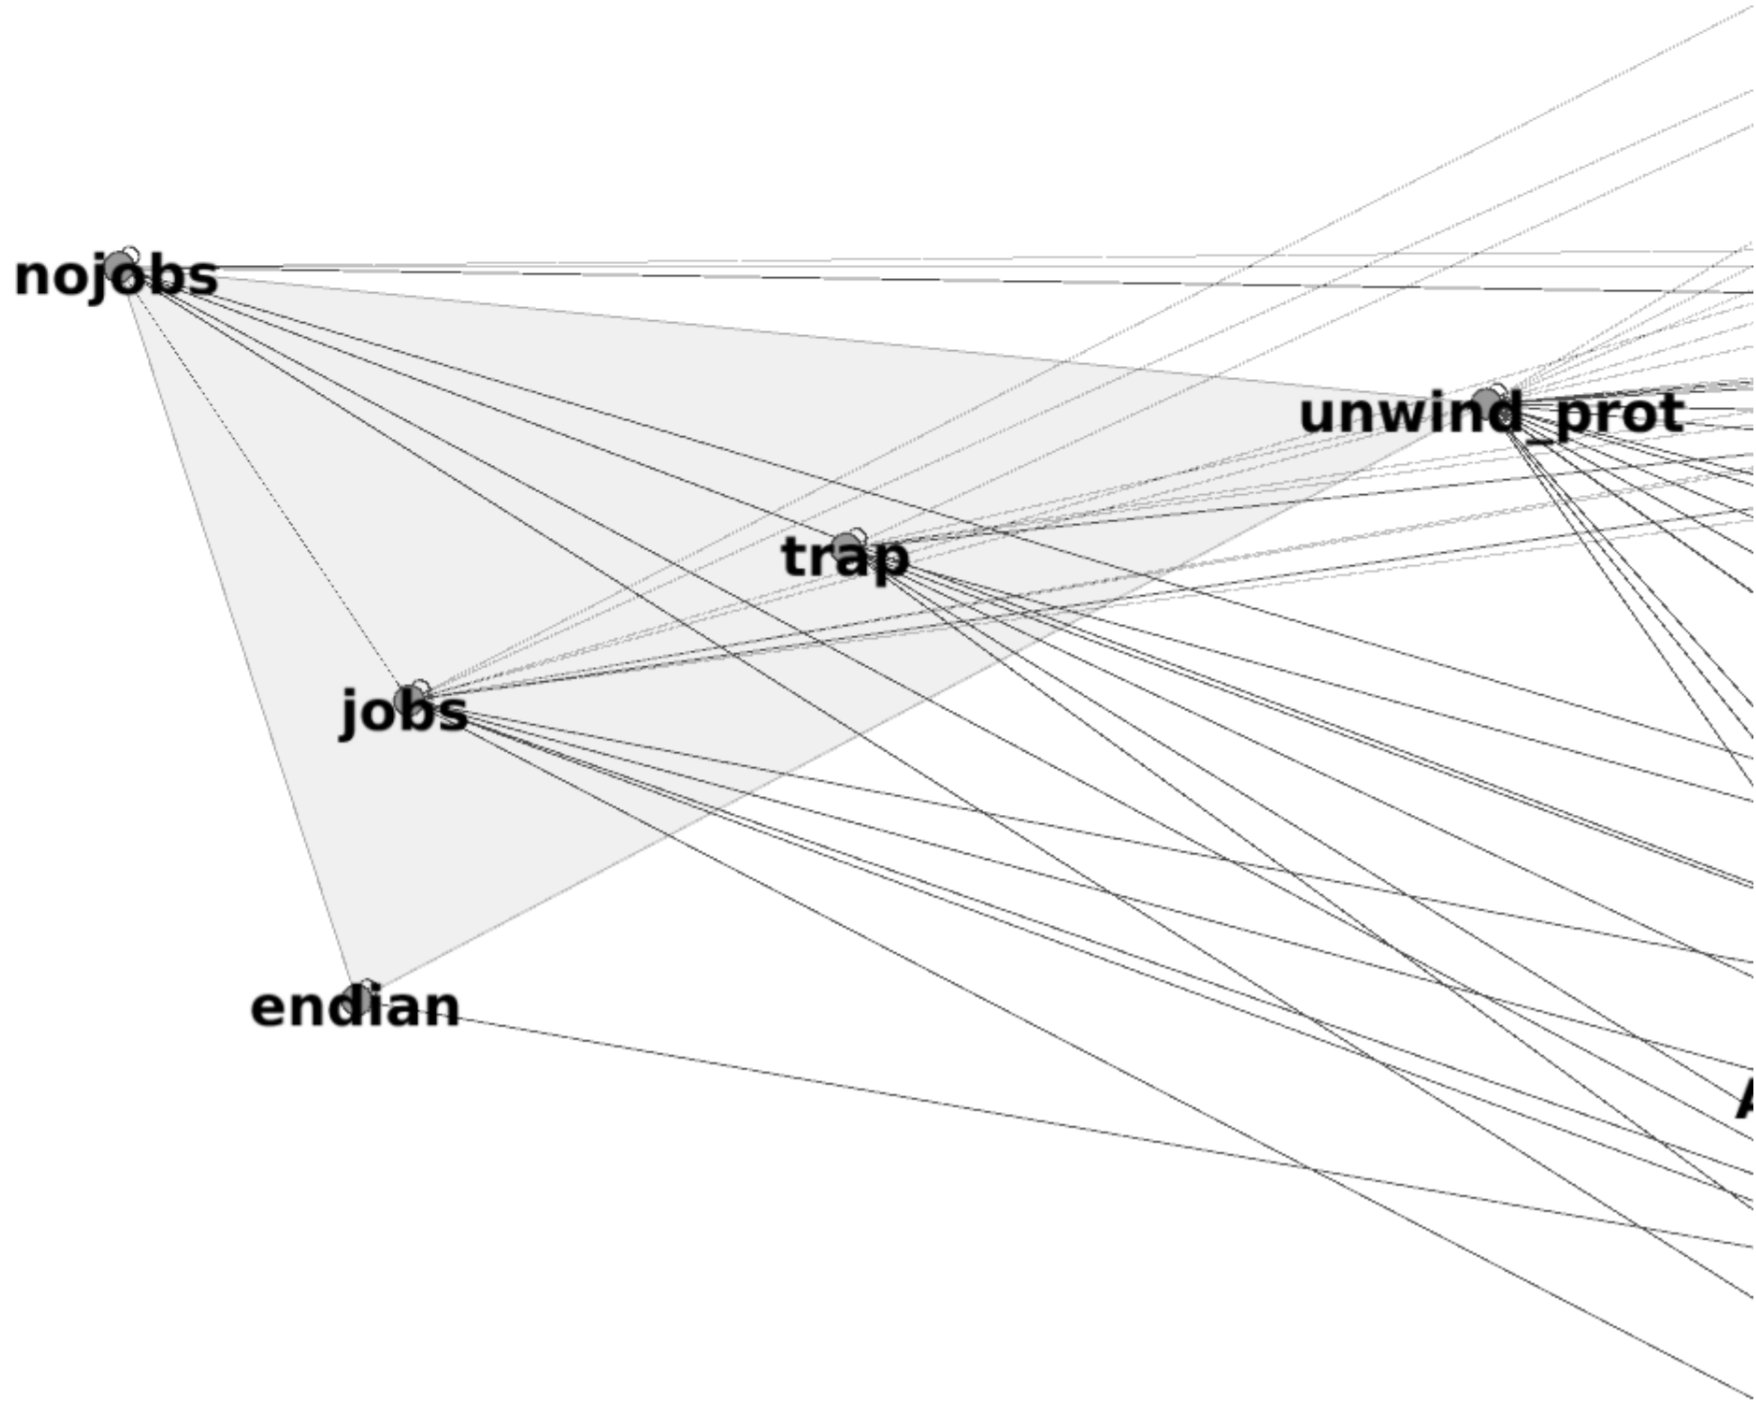
\includegraphics[width=0.7\textwidth]{bashJobControl.png}
        \end{center}
    \end{frame}

    \begin{frame}
        \frametitle{Commands}
        \begin{center}
            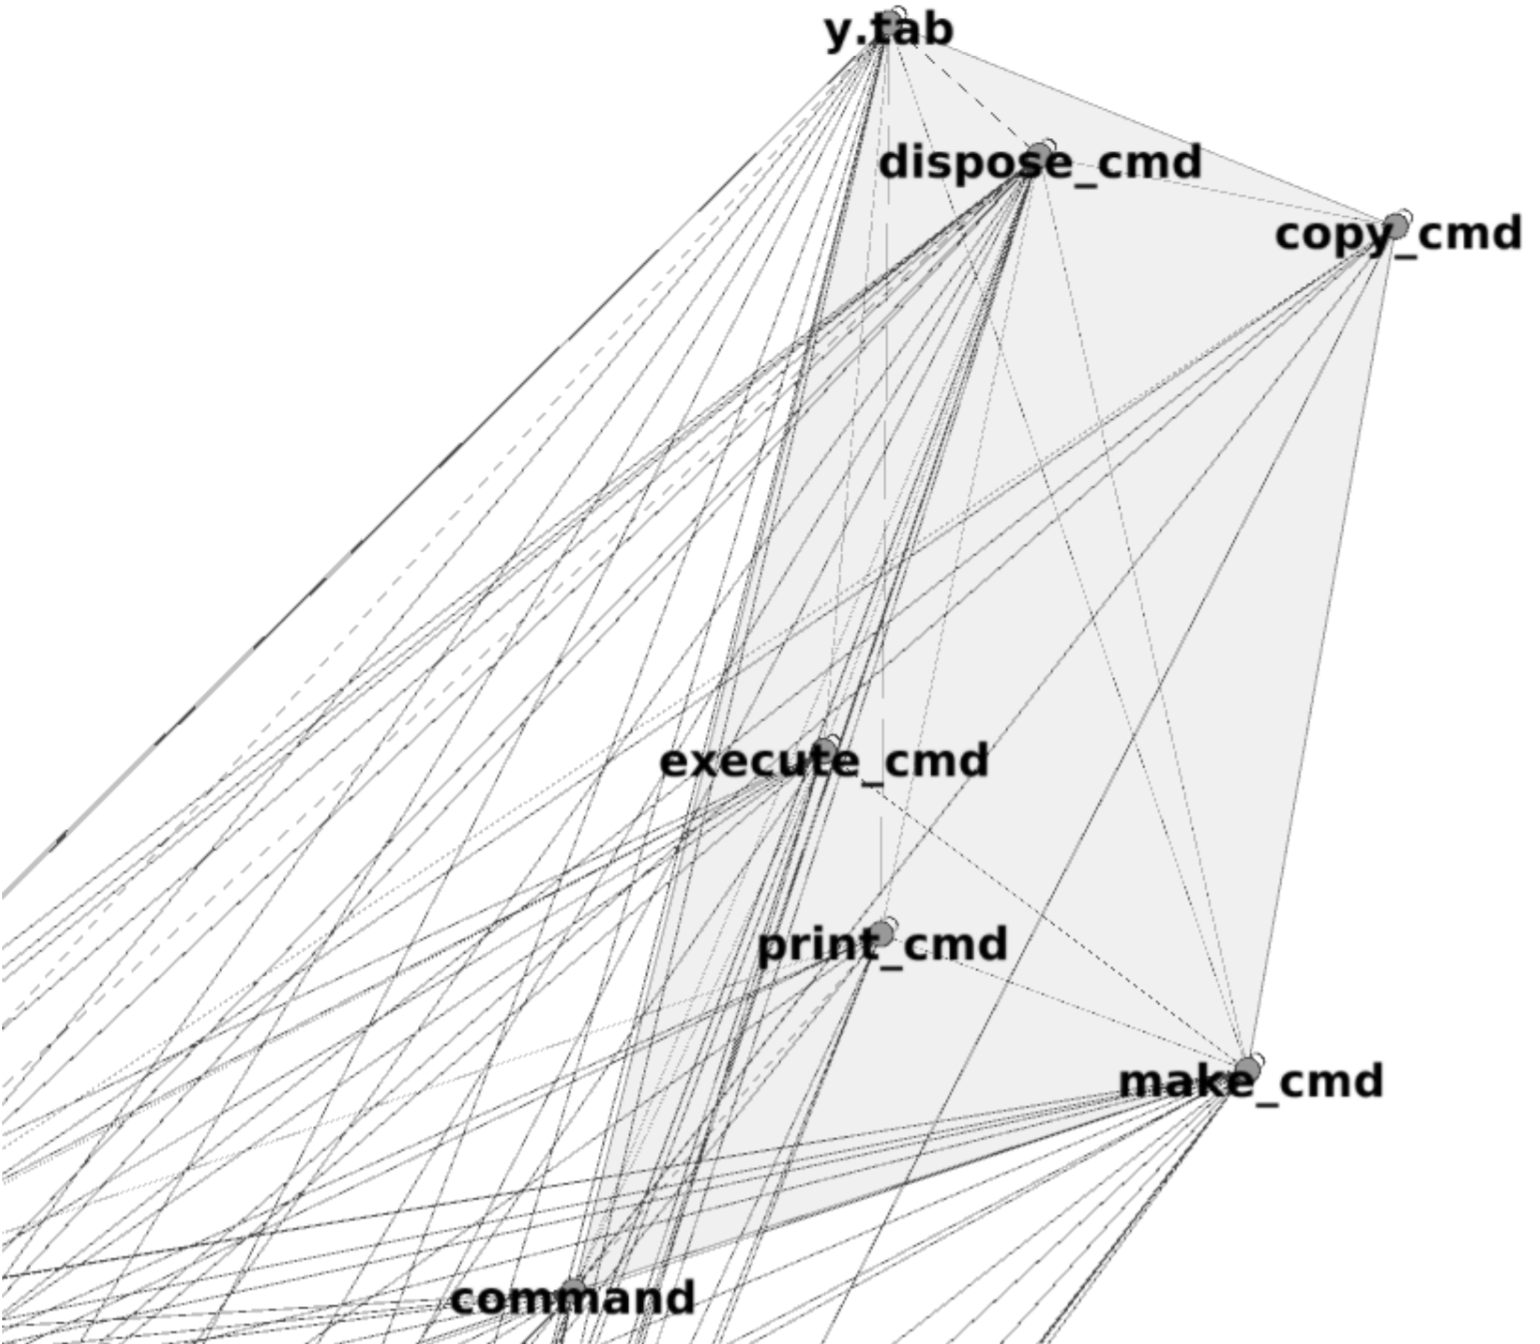
\includegraphics[width=0.7\textwidth]{bashCommands.png}
        \end{center}
    \end{frame}

    \section{Git}

    \begin{frame}
        \frametitle{Git\footnote{\tiny{По гл. 10 \url{https://git-scm.com/book} и \url{http://aosabook.org/en/git.html}}}}
        \begin{itemize}
            \item Распределённая VCS
            \item Linus Torvalds, 2005 год, драма с BitKeeper
            \item Architectural drivers
            \begin{itemize}
                \item Распределённая разработка с тысячей коммитеров
                \item Защита от порчи исходников
                \begin{itemize}
                    \item Возможность отменить мердж, смерджиться вручную
                \end{itemize}
                \item Высокая скорость работы
            \end{itemize}
        \end{itemize}
    \end{frame}

    \begin{frame}
        \frametitle{Внутреннее устройство Git}
        Структура папки .git:
        \begin{itemize}
            \item HEAD
            \item index
            \item config
            \item description
            \item hooks/
            \item info/
            \item objects/
            \item refs/
            \item ...
        \end{itemize}
    \end{frame}

    \begin{frame}[fragile]
        \frametitle{Объекты}
        Git внутри --- хеш-таблица, отображающая SHA-1-хеш файла в содержимое файла. Пример:
        \begin{minted}{text}
$ git init test
Initialized empty Git repository in /tmp/test/.git/
$ cd test
$ find .git/objects
.git/objects
.git/objects/info
.git/objects/pack

$ echo 'test content' | git hash-object -w --stdin
d670460b4b4aece5915caf5c68d12f560a9fe3e4

$ find .git/objects -type f
.git/objects/d6/70460b4b4aece5915caf5c68d12f560a9fe3e4
        \end{minted}
    \end{frame}

    \begin{frame}[fragile]
        \frametitle{Объекты (2)}
        Как получить сохранённый объект:
        \begin{minted}{text}
$ git cat-file -p d670460b4b4aece5915caf5c68d12f560a9fe3e4
test content
        \end{minted}

        Версионный контроль:
        \begin{minted}{text}
$ echo 'version 1' > test.txt
$ git hash-object -w test.txt
83baae61804e65cc73a7201a7252750c76066a30
$ echo 'version 2' > test.txt
$ git hash-object -w test.txt
1f7a7a472abf3dd9643fd615f6da379c4acb3e3a
$ find .git/objects -type f
.git/objects/1f/7a7a472abf3dd9643fd615f6da379c4acb3e3a
.git/objects/83/baae61804e65cc73a7201a7252750c76066a30
.git/objects/d6/70460b4b4aece5915caf5c68d12f560a9fe3e4
        \end{minted}
    \end{frame}

    \begin{frame}[fragile]
        \frametitle{Объекты (3)}
        Переключение между версиями файла:
        \begin{minted}{text}
$ git cat-file -p 83baae61804e65cc73a7201a7252750c76066a30 \
    > test.txt
$ cat test.txt
version 1

$ git cat-file -p 1f7a7a472abf3dd9643fd615f6da379c4acb3e3a \
    > test.txt
$ cat test.txt
version 2
        \end{minted}
    \end{frame}

    \begin{frame}[fragile]
        \frametitle{Деревья}
        blob (то, что мы видели раньше) хранит только содержимое файла, не хранит даже его имя. Решение проблемы --- tree:
        \begin{scriptsize}
        \begin{minted}{text}
$ git cat-file -p master^{tree}
100644 blob a906cb2a4a904a152e80877d4088654daad0c859      README
100644 blob 8f94139338f9404f26296befa88755fc2598c289      Rakefile
040000 tree 99f1a6d12cb4b6f19c8655fca46c3ecf317074e0      lib
        \end{minted}
        \end{scriptsize}
        \begin{center}
            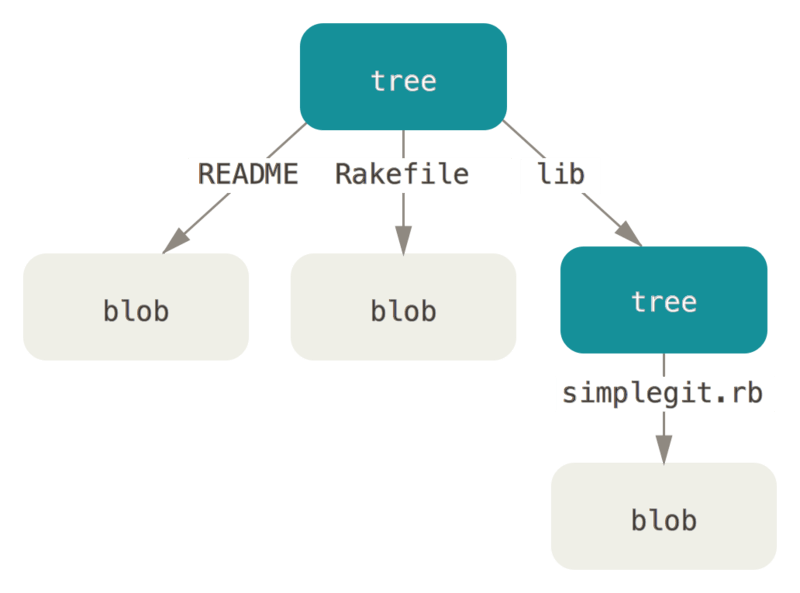
\includegraphics[width=0.5\textwidth]{gitTreeObject.png}
        \end{center}
    \end{frame}

    \begin{frame}
        \frametitle{Какие ещё виды объектов бывают}
        \begin{center}
            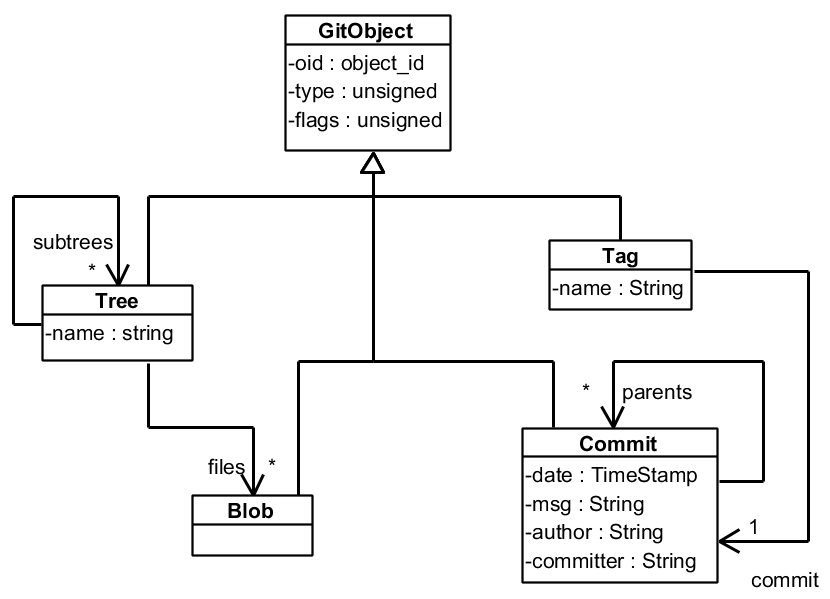
\includegraphics[width=0.7\textwidth]{gitDataStructure.png}
        \end{center}
    \end{frame}

    \begin{frame}[fragile]
        \frametitle{Коммиты}
        tree-объекты могут хранить структуру файлов (как inode в файловой системе), но не хранят метаинформацию типа автора файла и даты создания. Это хранится в commit-объектах:
        \begin{minted}{text}
$ echo 'first commit' | git commit-tree d8329f
fdf4fc3344e67ab068f836878b6c4951e3b15f3d

$ git cat-file -p fdf4fc3
tree d8329fc1cc938780ffdd9f94e0d364e0ea74f579
author Scott Chacon <schacon@gmail.com> 1243040974 -0700
committer Scott Chacon <schacon@gmail.com> 1243040974 -0700

first commit
        \end{minted}
        Ещё коммит хранит список коммитов-родителей
    \end{frame}

    \begin{frame}
        \frametitle{Коммиты, как это выглядит}
        \begin{center}
            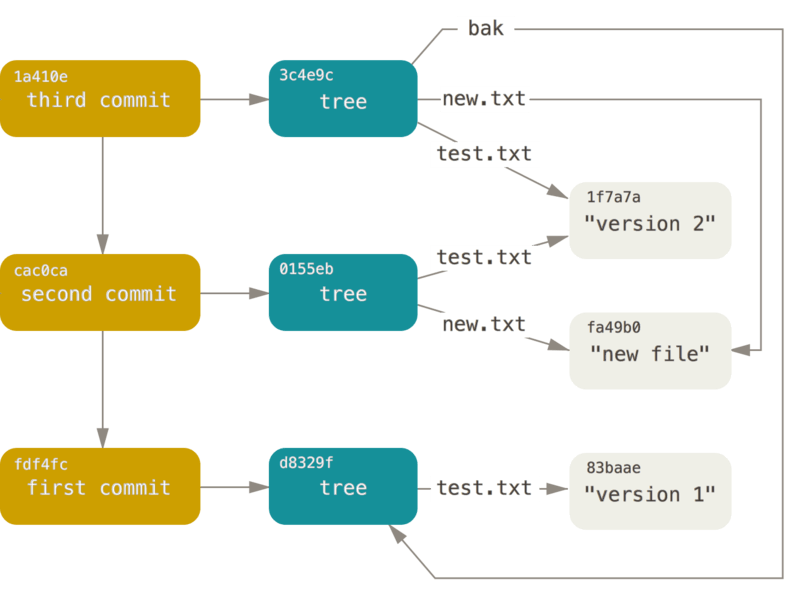
\includegraphics[width=0.7\textwidth]{gitCommitObjects.png}
        \end{center}
    \end{frame}

    \begin{frame}[fragile]
        \frametitle{Ссылки}
        Теперь вся информация хранится на диске, но чтобы ей воспользоваться, нужно помнить SHA-1 хеши. На помощь приходят reference-ы. 

        \begin{itemize}
            \item .git/refs
            \item .git/refs/heads
            \item .git/refs/tags
        \end{itemize}

        \begin{minted}{text}
$ echo "1a410efbd13591db07496601ebc7a059dd55cfe9" \
    > .git/refs/heads/master

$ git log --pretty=oneline master
1a410efbd13591db07496601ebc7a059dd55cfe9 third commit
cac0cab538b970a37ea1e769cbbde608743bc96d second commit
fdf4fc3344e67ab068f836878b6c4951e3b15f3d first commit
        \end{minted}
        \begin{itemize}
            \item Команда \verb|git update-ref|
        \end{itemize}
    \end{frame}

    \begin{frame}
        \frametitle{Ссылки, как это выглядит}
        \begin{center}
            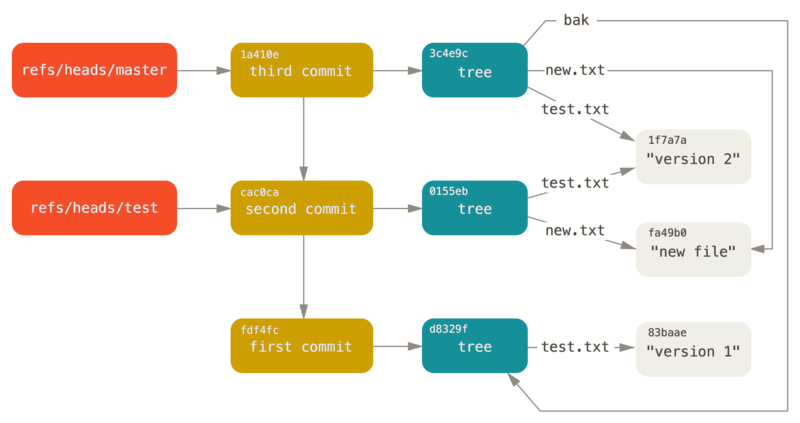
\includegraphics[width=0.9\textwidth]{gitRefs.png}
        \end{center}
    \end{frame}

    \begin{frame}[fragile]
        \frametitle{HEAD}
        Теперь не надо помнить хеши, но как переключаться между ветками?

        Текущая ветка хранится в HEAD. HEAD --- символическая ссылка, то есть ссылка на другую ссылку.
        \begin{minted}{text}
$ cat .git/HEAD
ref: refs/heads/master

$ git symbolic-ref HEAD refs/heads/test
$ cat .git/HEAD
ref: refs/heads/test
        \end{minted}
    \end{frame}

    \begin{frame}[fragile]
        \frametitle{Тэги}
        Последний из объектов в Git --- tag. Это просто указатель на коммит.
        \begin{footnotesize}
            \begin{itemize}
                \item Легковесный тэг:
                    \begin{minted}{text}
git update-ref refs/tags/v1.0 cac0cab538b970a37ea1e769cbbde608743bc96d
                    \end{minted}
                    Или просто git tag
                \item Аннотированный тэг:
                    \begin{minted}{text}
$ git tag -a v1.1 1a410efbd13591db07496601ebc7a059dd55cfe9 -m 'test tag'

$ git cat-file -p 9585191f37f7b0fb9444f35a9bf50de191beadc2
object 1a410efbd13591db07496601ebc7a059dd55cfe9
type commit
tag v1.1
tagger Scott Chacon <schacon@gmail.com> Sat May 23 16:48:58 2009 -0700

test tag
                    \end{minted}
            \end{itemize}
        \end{footnotesize}
    \end{frame}

    \begin{frame}[fragile]
        \frametitle{Packfiles}
        Пока что получалось, что все версии всех файлов в Git хранятся целиком, как они есть. Все они всегда сжимаются zlib, но в целом, если создать репозиторий, добавлять туда файлы, коммитить и т.д., все версии всех файлов будут в нём целиком. На помощь приходят .pack-файлы:
        \begin{footnotesize}
            \begin{minted}{text}
$ git gc
Counting objects: 18, done.
Delta compression using up to 8 threads.
Compressing objects: 100% (14/14), done.
Writing objects: 100% (18/18), done.
Total 18 (delta 3), reused 0 (delta 0)

$ find .git/objects -type f
.git/objects/bd/9dbf5aae1a3862dd1526723246b20206e5fc37
.git/objects/d6/70460b4b4aece5915caf5c68d12f560a9fe3e4
.git/objects/info/packs
.git/objects/pack/pack-978e03944f5c581011e6998cd0e9e30000905586.idx
.git/objects/pack/pack-978e03944f5c581011e6998cd0e9e30000905586.pack
            \end{minted}
        \end{footnotesize}
    \end{frame}

    \begin{frame}
        \frametitle{Как оно устроено}
        \begin{center}
            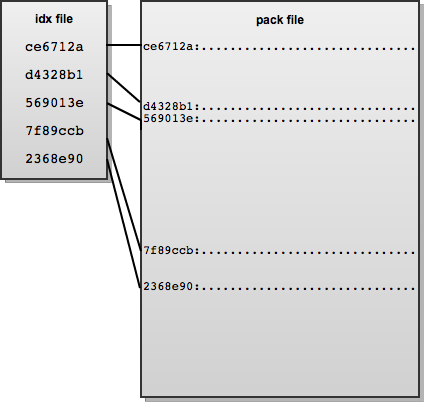
\includegraphics[width=0.6\textwidth]{gitPackFiles.png}
        \end{center}
    \end{frame}

    \begin{frame}
        \frametitle{Pack-файлы, подробности}
        \begin{itemize}
            \item Упаковка происходит, когда:
            \begin{itemize}
                \item Выполняется git push
                \item Слишком много <<свободных>> объектов (порядка 7000)
                \item Вручную вызвана git gc
            \end{itemize}
            \item Используется дельта-компрессия
            \begin{itemize}
                \item Последняя версия хранится целиком, дельты <<идут назад>>
            \end{itemize}
            \item Можно заглянуть внутрь, git verify-pack
            \item Git может хитро перепаковывать pack-файлы
        \end{itemize}
    \end{frame}

    \begin{frame}[fragile]
        \frametitle{Reflog и восстановление коммитов}
            \begin{minted}{text}
$ git reflog
1a410ef HEAD@{0}: reset: moving to 1a410ef
ab1afef HEAD@{1}: commit: modified repo.rb a bit
484a592 HEAD@{2}: commit: added repo.rb

$ git log -g
commit 1a410efbd13591db07496601ebc7a059dd55cfe9
Reflog: HEAD@{0} (Scott Chacon <schacon@gmail.com>)
Reflog message: updating HEAD
Author: Scott Chacon <schacon@gmail.com>
Date:   Fri May 22 18:22:37 2009 -0700

    third commit
$ git branch recover-branch ab1afef
            \end{minted}
    \end{frame}

    \begin{frame}[fragile]
        \frametitle{Как более капитально прострелить себе ногу}
        \framesubtitle{И что делать}
        \begin{minted}{text}
$ git branch -D recover-branch
$ rm -Rf .git/logs/

$ git fsck --full
Checking object directories: 100% (256/256), done.
Checking objects: 100% (18/18), done.
dangling blob d670460b4b4aece5915caf5c68d12f560a9fe3e4
dangling commit ab1afef80fac8e34258ff41fc1b867c702daa24b
dangling tree aea790b9a58f6cf6f2804eeac9f0abbe9631e4c9
dangling blob 7108f7ecb345ee9d0084193f147cdad4d2998293
        \end{minted}
        Git не удалит даже <<висячие>> объекты несколько месяцев, если его явно не попросить.
    \end{frame}

    \begin{frame}
        \frametitle{Lessons Learned}
        \begin{itemize}
            \item Команды реализовывались как набор шелл-скриптов
            \begin{itemize}
                \item Не портировать под Windows
                \item Сложно интегрировать с IDE
                \item Замедлило внедрение git-а
            \end{itemize}
            \item Большой набор команд (включая plumbing) делает Git тяжёлым для изучения и усложняет сообщения об ошибках
        \end{itemize}
    \end{frame}

    \section{Wesnoth}

    \begin{frame}
        \frametitle{Battle for Wesnoth\footnote{\tiny{По \url{http://aosabook.org}}}}
        \begin{columns}
            \begin{column}{0.4\textwidth}
                \begin{itemize}
                    \item Пошаговая стратегия
                    \item Порядка 200000 строк кода на C++
                    \item 4 миллиона скачиваний
                    \item 9/10 на Steam
                    \item 2003 год
                \end{itemize}
            \end{column}
            \begin{column}{0.6\textwidth}
                \includegraphics[width=\textwidth]{wesnoth.png}
                \attribution{https://www.wesnoth.org/}
            \end{column}
        \end{columns}
    \end{frame}

    \begin{frame}
        \frametitle{Architectural Drivers}
        \begin{itemize}
            \item Доступность для новых разработчиков и авторов контента
            \item В ущерб технической красоте
            \item Не nice to have, а условие выживания проекта в контексте широкого open-source сообщества из людей без каких-либо обязательств и разного технического уровня
        \end{itemize}
    \end{frame}

    \begin{frame}
        \frametitle{Высокоуровневая архитектура}
        \begin{columns}
            \begin{column}{0.6\textwidth}
                \begin{itemize}
                    \item Wesnoth Markup Language (WML)
                    \item Минимизация зависимостей от сторонних библиотек
                    \begin{itemize}
                        \item SDL (Simple Directmedia Layer) для видео и ввода/вывода
                        \begin{itemize}
                            \item Простота использования и кроссплатформенность
                        \end{itemize}
                        \item Boost, Pango, zlib, Python, Lua, GNU gettext
                    \end{itemize}
                \end{itemize}
            \end{column}
            \begin{column}{0.4\textwidth}
                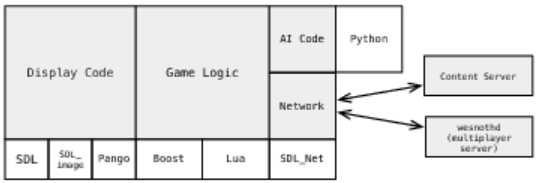
\includegraphics[width=\textwidth]{wesnothArchitecture.png}
            \end{column}
        \end{columns}
    \end{frame}

    \begin{frame}
        \frametitle{Основные компоненты}
        \begin{itemize}
            \item Парсер и препроцессор WML
            \item Базовый ввод-вывод --- видео, звук, сеть
            \item GUI --- виджеты
            \item Display module --- игровая доска, юниты, анимация и т.д.
            \item ИИ
            \item Поиск пути (плюс утилиты для работы с гексагональной доской)
            \item Генератор карт
            \item Специализированные модули
            \begin{itemize}
                \item Титульный экран
                \item Storyline module --- для проигрывания катсцен
                \item Лобби --- для мультиплеера
                \item ``Play game'' module --- управление основным игровым процессом
            \end{itemize}
            \item Отдельно --- wesnothd и content server
        \end{itemize}
    \end{frame}

    \begin{frame}[fragile]
        \frametitle{Wesnoth Markup Language}
        \begin{minted}{text}
[unit_type]
    id=Elvish Fighter
    name= _ "Elvish Fighter"
    image="units/elves-wood/fighter.png"
    hitpoints=33
    advances_to=Elvish Captain,Elvish Hero
    {LESS_NIMBLE_ELF}
    [attack]
        name=sword
        icon=attacks/sword-elven.png
        range=melee
        damage=5
    [/attack]
[/unit_type]
        \end{minted}
    \end{frame}

    \begin{frame}[fragile]
        \frametitle{Макросы}
        \begin{minted}{c++}
#define GOLD EASY_AMOUNT NORMAL_AMOUNT HARD_AMOUNT
  #ifdef EASY
    gold={EASY_AMOUNT}
  #endif
  #ifdef NORMAL
    gold={NORMAL_AMOUNT}
  #endif
  #ifdef HARD
    gold={HARD_AMOUNT}
  #endif
#enddef
...
{GOLD 50 100 200}
        \end{minted}
    \end{frame}

    \begin{frame}
        \frametitle{Модель данных}
        \begin{itemize}
            \item Всё сливается в один гигантский WML-документ
            \item Перезагружается при смене опций
            \item Всякие хаки на уровне препроцессора, чтобы не грузить вообще всё
            \item Классы unit и unit\_type (архитектурный стиль Knowledge Layer)
            \item Фиксированный набор поддерживаемых движком атрибутов, задаваемых для каждого типа через WML
            \begin{itemize}
                \item Нельзя описывать произвольное поведение через WML, хотели сохранить декларативность
            \end{itemize}
            \item Класс attack\_type
            \item Трейты, инвентарь
        \end{itemize}
    \end{frame}

    \begin{frame}
        \frametitle{Мультиплеер}
        \begin{itemize}
            \item Начальное состояние и команды
            \item Сервер просто пересылает команды между клиентами
            \begin{itemize}
                \item TCP/IP
            \end{itemize}
            \item Replay
            \item Никакой защиты от читов
            \item Версии клиентов
        \end{itemize}
    \end{frame}

    \begin{frame}
        \frametitle{Lessons Learned}
        \begin{itemize}
            \item 250 тысяч строк на WML
            \item Сотни созданных пользователями кампаний
            \item 74 тысячи коммитов, 196 контрибуторов
            \item Сами разработчики смеются над WML
            \item В целом задача обеспечить доступность для модификации очень сложна
        \end{itemize}
    \end{frame}

\end{document}
